% vim: set fenc=utf-8 ft=latex encoding=utf-8
% -*- mode: latex; coding: UTF-8; -*-
%!TEX root = knowledge-curation.tex
\section{Methodology}
\label{cha:methodology}

As mentioned, the main goal of this work is to empirically compare how knowledge, specifically knowledge in question-and-answer (Q\&A) form, is sought, shared, and curated in both the \RH mailing list and the R tag on \SO. We used a qualitative \textit{exploratory case study} methodology~\cite{Creswell2009,Runeson2012} to answer our research questions (presented in Section~\ref{cha:introduction}).
    % \begin{enumerate}[label=\bfseries{RQ\arabic*.},itemsep=3pt, topsep=2pt, leftmargin=3em, parsep=0pt]
    %     \item \rqa
    %     \item \rqb
    %     \item \rqc
    %  \end{enumerate}

%We performed a qualitative case study~\cite{Creswell2009,Runeson2012} of the knowledge that flows through both \RH and \SO.
%This research method is applicable when a concept or phenomenon requires more understanding, with little pre-existing research~\cite{Creswell2009}.

This study employed two research methods over two phases: we \textit{mined archival data} and then conducted a \textit{qualitative survey}. In the first phase,
we randomly sampled and iteratively coded\footnote{Our sample data is openly available at \url{https://zenodo.org/record/47484}} questions in both channels to characterize the types of discussions that occur~\cite{carlos_gomez_teshima_2016_47484}. This process was continued until we reached saturation, which amounted to 400 threads in each channel. In the second phase, we surveyed members of the R community to validate our interpretation of the results from the previous phase. %obtain further additional insights and to verify our findings.

\subsection{Phase I: Mining Archival Data} 
\label{sec:studyDesign}
We mined data from the public archives of both the \RH mailing list and \SO. The \RH mailing list archive started in 1997, while the archives for \SO started in 2008 (when it was created).
To make the data sets comparable, we analyzed both datasets from September 2008 until December 2013, a period of time that both channels were available.
For \SO, we obtained a data dump file from their Website---Stack Exchange releases a new data dump from all their Websites every three months\footnote{\url{http://stackexchange.com/sites}}. For the \RH mailing list data, we retrieved MBOX files of the archives from the \RH Website.

%To make the data comparable againt the \SO data set, we transformed the email addresses to MD5 hashes, and changed the time zone of the mailing list messages (UTC+2) to the time zone used by \SO (UTC).
    
To answer RQ3, we needed the ability to compare email addresses between both channels. However, Stack Exchange stopped providing information about email addresses and the last Stack Exchange dump file to contain email addresses as MD5 hashes was released in September 2013---this meant we did not have complete data for October, November, and December 2013. 
To remedy this gap, we used the data dump file from September 2014, but updated the \texttt{users} table with the hashes taken from the September 2013 dump file for those \texttt{ID}s that were identical in both data sets.
However, if a user in the 2013 data file did not exist in the 2014 data, we did not count them.
From \SO, we retrieved all R-related data by selecting only messages that contained the R tag (\texttt{r}) or its two synonyms\footnote{\url{http://stackoverflow.com/tags/r/synonyms}}, (\texttt{rstats} and \texttt{r-language}).

To determine which users were active in both channels, we compared the MD5 hashes of the \RH mailing list and \SO participants. Given the limitations of the \SO data, we did not perform any unification of email addresses and considered that every email address belonged to an individual. In total, we found 1,421 active users (email addresses) on both media channels.

    % Although MD5 hashes are not \textit{collision resistant} and could possibly lead to false positives, it is unlikely that two different email addresses share a MD5 hash.

To prepare the data, we used two different software tools:
    \begin{enumerate*}[label=(\arabic*)]
    \item To process the \SO data, we used a modified version of Sam Saffron's application, So-Slow\footnote{\url{https://github.com/SamSaffron/So-Slow}}.
    \item To process the \RH mailing list data, we wrote our own mail mining application\footnote{Our tool is available at
            \url{https://github.com/cagomezt/GTMail}}. To ensure accurate results when processing the \RH mailing list, we followed a series of recommendations proposed by Bettenburg \textit{et al.}~\cite{Bettenburg2009}: extracted messages, removed duplicates, removed signatures, and reconstructed discussion threads.
    \end{enumerate*}
Table~\ref{table:data} depicts a summary of the data used for this study. Unsurprisingly, the \RH mailing list has more questions, answers, and users as it contains approximately ten years of additional data.
Note that only \SO's data contains ``comments'' information.

	\begin{table}[!htb]
	  \centering
      \caption{Raw data collected for each channel.}
      \begin{small}
        \begin{tabular}{lrr}
	        \toprule
	        Type          &  \RH & \SO \\
	        \midrule
	        Questions     & 101,931 &  67,393 \\
	        Answers       & 213,366 &  99,620 \\
	        Comments      &       - & 286,124 \\
	        Users         &  39,150 &  26,324 \\
	        \bottomrule
        \end{tabular}
      \end{small}
	  \label{table:data}
	\end{table}





\subsubsection{Data analysis process}
\label{sec:dap}

We followed an inductive approach~\cite{Runeson2012} to analyze the data from \SO and the \RH mailing list. 
% MS: this contradicts the following sentence about selecting 400 messages... perhaps you iterated on the analysis but you selected the 400 messages from each channel to start with.  I'm rewording it. 
% Through this process, we iteratively switched between \textit{data gathering} and \textit{data analysis} until we reached saturation. 
%
To reduce the risk of bias~\cite{Runeson2012}, the analysis was conducted by two computer scientists with a background in qualitative data analysis.
 To answer RQ1 and RQ2, we selected 400 random threads from each channel. To answer RQ3, we focused on questions with identical subjects that were posted to both channels by the same author---we found and analyzed 79 such threads.
    
    \begin{figure*}[htbp]
    	\centering
    	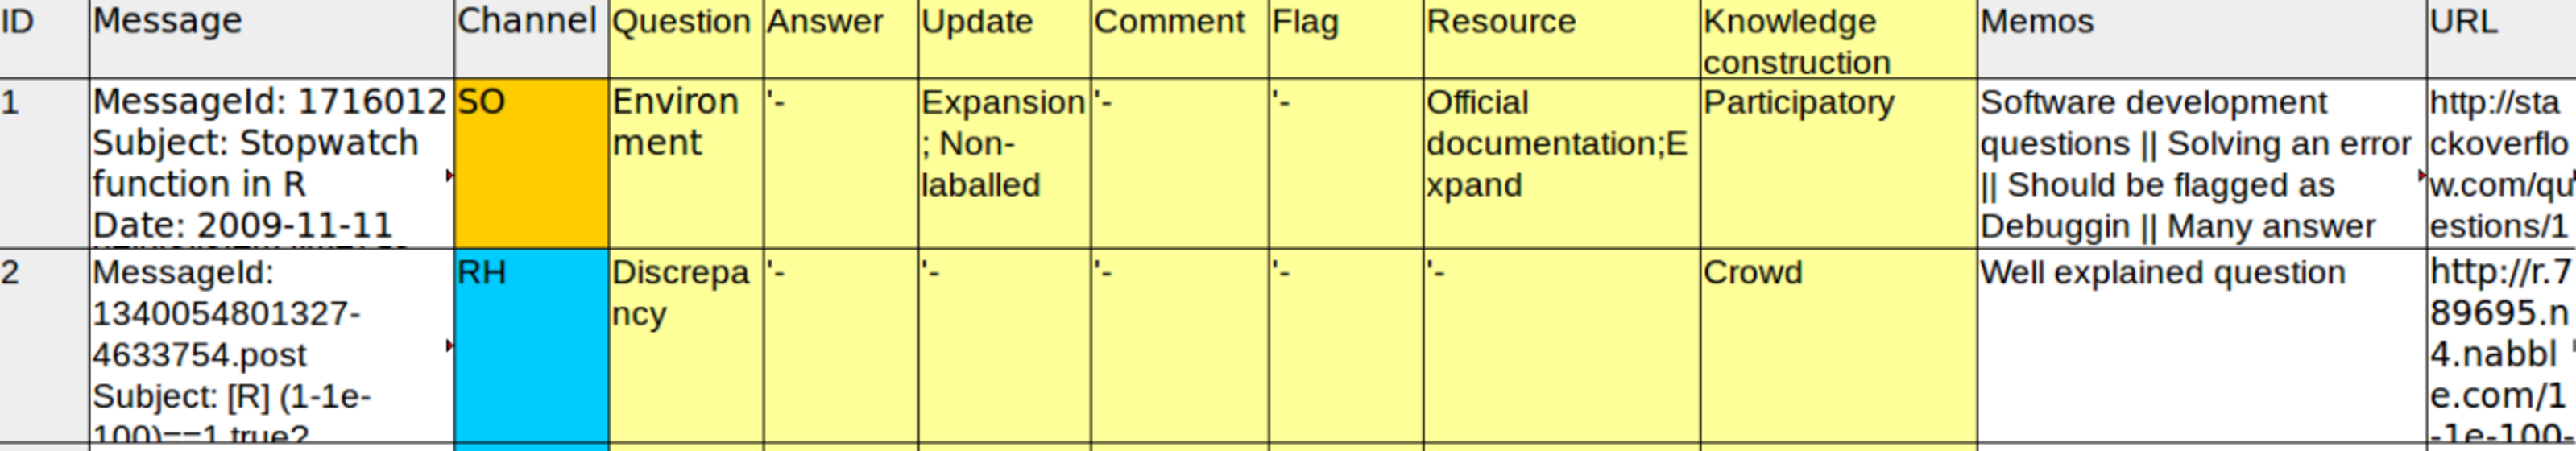
\includegraphics[width=.95\textwidth]{Figures/CodingExample}
    	\caption{Example of data coding. Each row is a threaded message. Questions, comments, and answers are identified with the number on the first column. Columns in yellow (columns 4-10) contain the code for each message type. The last two columns contain the memos and the URL.}
    	\label{fig:CodingExample}
%\vspace{-3mm}
    \end{figure*}

We used \textbf{memoing}, \textbf{affinity diagrams}, and a \textbf{code book} to support the data analysis process. We wrote reflective memos in a spreadsheet next to the applicable codes (see example in Fig.~\ref{fig:CodingExample}). These memos were used to create the codes and hypotheses about the relationships between concepts. We coded in multiple sessions, which allowed us to refine the definitions in the code book 
%MS: this is new to reflect iteration and saturation:
in an iterative manner. Each entry is associated with a title, a formal definition, an example, and notes from the researchers. %The final version of the code book is detailed in section~\ref{cha:findings}.
% MS:  ideally we should say how long it took to finalize the codes... and how this was done... I don't recall... 
For inter-rater reliability, we used the Cohen Kappa \textbf{inter-rater agreement} coefficient~\cite{Stemler2004}. Although it is suggested that one should aim for coefficient values above 0.6 to obtain substantial results~\cite{Landis1977}, based on our previous experience with this method~\cite{Gomez2013}, we aimed for 0.8 or above. We used this coefficient after each coding session as a way to trigger discussion and to further refine the codes if necessary.  
% MS: this is new:
The emergent codes were fully saturated after reviewing 400 threads from each channel. 


	% \begin{description}[itemsep=2pt, topsep=0pt, leftmargin=1em, parsep=0pt]
	% 	\item[Memoing] is the act of taking notes (coding) on what the researcher is learning from the data during the analysis~\cite{Groenewald2008}.
 %        We wrote reflective memos in a spreadsheet next to the applicable codes (see figure \ref{fig:CodingExample}).
 %        These memos were used to create the codes, and hypotheses about the relationships between concepts.

	% 	\item[Affinity diagrams] allows to organize ideas and data into groups, and to find the relationships between concepts~\cite{Scupin1997}.
	% 	We used them to discuss new insights, and while defining categories and relationships between them.

	% 	\item[Inter-rater agreement \textit{Cohen Kappa}] is a coefficient used to measure the agreement between two coders who classify items into mutually exclusive categories~\cite{Stemler2004}.
	% 	Ladis and Koch suggest that values above 0.60 or 60\% to obtain substantial results~\cite{Landis1977}.
	% 	In a previous study~\cite{Gomez2013}, we used the same coefficient to measure agreement between coders.
	% 	Based on this experience, we set a value above 0.80 or 80\% as the minimum to obtain substantial results.
	% 	We used this coefficient after each coding session as a way to trigger discussion.

	% 	\item[Code book] is a book that contains the definitions of the codes that researchers look during the data analysis~\cite{MacQueen1998}.
	% 	We coded in multiple sessions, which allowed us to refine the definitions.
	% 	Each entry is associated with a title, a formal definition, an example, and space for notes from the researcher.
	% 	The final version of the code book is detailed in section~\ref{cha:findings}.
	% \end{description}

The analysis process required an \textit{understanding of the context} surrounding each message. The process consisted of: (1) gathering the required information from each channel (i.e., the message analyzed, the relevant thread), and (2) mapping the messages from each channel to a specific knowledge type (see Section~\ref{cha:findings-types}). The mapping was necessary as each channel contained a different data structure.
We defined the following mappings between messages in both channels:

	\begin{description}[itemsep=1pt, topsep=2pt, leftmargin=1em, parsep=0pt]
		\item[Question:] The message is the first in the thread and contains the main question.
		\item[Answer:] The message provides a solution to the main question of the thread.
	 	\item[Update:] The message requests a modification to a question or answer made by the author of said question or answer.
		\item[Comment:] The message offers clarification to a specific part of the question or answer.
		\item[Flag:] The message requests attention from the moderator (e.g., repeated questions, spam, or rude behavior).
	\end{description}

%	The data set was capped at 400 threads for each channel when we deemed our observations as being saturated.

\subsection{Phase II: Qualitative Survey}

The analysis from Phase I revealed that some developers are active on both channels, and in some cases, even post the same questions. To further understand this phenomena and explore the perceived benefits of using one channel over the other, we conducted a survey with members of the R community\footnote{A copy of the survey is available at \url{http://goo.gl/mxmH5J}}. % in order to validate our interpretation of the results from Phase I. %with the purpose of obtaining additional insights on the findings.

To test and refine the questions, format, and tone, we piloted the survey twice. 
We promoted our survey on Twitter, Reddit, the \RH mailing list, and Meta Stack Exchange to reach users of both channels and minimize selection bias. However, our survey invitation on Stack Exchange was deemed off topic and deleted a few minutes later. In total, we received 37 responses, 26 of which were valid (invalid responses occurred if the session ended or the participant did not complete the survey).

%%% Local Variables:
%%% mode: latex
%%% TeX-master: "knowledge-curation.tex"
%%% End:
